% ==========================================
% EXPERIMENTS AND RESULT
% ==========================================

\newpage
\chapter{THÍ NGHIỆM, ĐÁNH GIÁ VÀ KẾT LUẬN}

\section{Thí nghiệm và đánh giá kết quả}

\subsection{Kế hoạch thực hiện thí nghiệm}

\hspace{0.5cm}Công việc thực hiện thí nghiệm để có thể phân tích và nhận dạng packer được chia làm các bước sau:

\begin{itemize}
\item{Để có thể thí nghiệm phân tích packer trên hệ thống BE-PUM. Lựa chọn 9 tập tin mẫu và nén bằng 27 packer. Các tập tin mẫu bao gồm 5 tập tin tự tạo: api\_test.exe, demo1.exe, demo2.exe, bof.exe, api\_test\_v2.exe và 4 virus trong thực tế từ tập virus VXHeaven bao gồm: Virus.Win32.Aztec, Virus.Win32.Adson, Virus.Win32.Benny và Virus.Win32.Cabanas.2999.\\}
\item{Để có thể thí nghiệm nhận dạng packer qua kết hợp giữa hệ thống BE-PUM và công cụ NuSMV, lựa chọn từ tập virus LORIA 2000 virus và tiến hành chạy tự động.\\} 
\item{Để có thể đưa ra so sánh giữa hai phương pháp nhận dạng packer, một là thông qua phương pháp nhận dạng chữ ký và hai là phương pháp nhận dạng thông qua model checking. Thí nghiệm về nhận dạng packer thông qua chữ ký cũng sẽ được tiến hành.}
\end{itemize}

\hspace{0.5cm}Thí nghiệm được thực hiện trên hệ thống VMWare WinXP SP3, Intel Core i5 - 2450M 2.5GHz, 2GB RAM, JDK 1.8 và công cụ thực hiện kiểm tra mô hình NuSMV 2.6.0.

\subsection{Kết quả thí nghiệm}

\hspace{0.5cm}Kết quả thí nghiệm phân tích packer trên hệ thống BE-PUM được thể hiện trong bảng \ref {tab:27PackerExp}, bao gồm các 27 packer đã được hệ thống BE-PUM phân tích hoàn toàn, cũng như số node và edge được sinh ra sau khi phân tích các packer này.

\begin{small}
\setlength\tabcolsep{3pt}
\centering
\begin{longtable}{|l|l|l|l|}
\hline
\textbf{Tập tin nén api\_test.exe}	& \textbf{Nodes}	& \textbf{Edges}	& \textbf{Time}	\\
\hline 
ASPACK								& 1047				& 1112				& 58969 		\\
\hline 	
BJFNT								& 2061				& 2126				& 2810453		\\
\hline 
EXEPACK								& 323				& 353				& 6719			\\
\hline 
EXESTEALTH							& 735				& 770				& 238438		\\
\hline 
EXPRESSOR							& 1172				& 1233				& 76797			\\
\hline 
FSG									& 244				& 268				& 4000			\\
\hline 
LAME								& 235				& 244				& 10062			\\
\hline 
MEW									& 110				& 131				& 3187			\\
\hline 
MORPHNAH							& 228				& 232				& 3593			\\
\hline 
MPRESS								& 459				& 489				& 101391		\\
\hline 
NOODLECRYPT							& 706				& 757				& 33922			\\
\hline 
NPACK								& 602				& 639				& 9609			\\
\hline 
PECOMPACT							& 1127				& 1178				& 30891			\\
\hline 
PEECRYPT							& 511				& 517				& 26750			\\
\hline 
PETITE								& 1568				& 1635				& 49593			\\
\hline 
RLPACK								& 467				& 501				& 265937		\\
\hline 
SCRAMBLE v0.1						& 266				& 292				& 3984			\\
\hline 
SCRAMBLE v0.2						& 244				& 268				& 3922			\\
\hline 
TELOCK								& 2105				& 2237				& 6276360		\\
\hline 
UPACK								& 443				& 490				& 19625			\\
\hline 
UPX									& 323				& 353				& 6875			\\
\hline 
WINUPACK							& 443				& 490				& 19734			\\
\hline 
WWPACK32							& 329				& 360				& 3219			\\
\hline 
XCOMP								& 650				& 724				& 224734		\\
\hline 
YODA v1.2							& 625				& 659				& 130500		\\
\hline 
YODA v1.3							& 924				& 960				& 120516		\\
\hline 
PELOCK								& 2032				& 2033				& 36903693		\\
\hline 
PESPIN								& 431				& 452				& 4860547		\\
\hline
\caption {Kết quả thí nghiệm trên 27 packer}\label{tab:27PackerExp}
\end{longtable}
\end{small}

\hspace{0.5cm}Kết quả thí nghiệm nhận dạng 14 kỹ thuật trên 27 packer qua việc kết hợp giữa hệ thống BE-PUM và công cụ NuSMV được thể hiện trong bảng \ref {tab:27PackerSemanticExp}.

\begin{tiny}
\setlength\tabcolsep{1pt}
\centering
\begin{longtable}{|l|c|c|c|c|c|c|c|c|c|c|c|c|c|c|}
\hline
\textbf{Packer}	& \textbf{\specialcell{Anti\\Debu\\gging}}	& \textbf{\specialcell{Check\\summ-\\ing}}	& \textbf{\specialcell{Code\\Chunk-\\ing}}		& \textbf{\specialcell{Indi-\\rect\\Jump}}		& \textbf{\specialcell{Obfus-\\cated\\Const-\\ants}}		& \textbf{\specialcell{Over-\\lapp-\\ing\\Block}}		& \textbf{\specialcell{Over-\\lapp-\\ing\\Func-\\tion}}		& \textbf{\specialcell{Over-\\writt-\\ing}}		& \textbf{\specialcell{Pack-\\ing\\Un-\\pack-\\ing}}	& \textbf{\specialcell{SEH}}	& \textbf{\specialcell{Stolen\\Bytes}}		& \textbf{\specialcell{Timm-\\ing\\Check}}		& \textbf{\specialcell{Two\\APIs}}		& \textbf{\specialcell{Hard-\\ware\\Break-\\points}} \\
\hline 
ASPACK				&	&x	&x	&x	&x	&x	&x	&x	&x	&	&x	&	&	&	\\
\hline
BJFNT				&	&x	&x	&	&x	&x	&	&x	&x	&	&	&	&	&	\\
\hline
EXEPACK				&	&x	&	&x	&x	&x	&	&x	&x	&	&	&	&x	&	\\
\hline
EXESTEALTH			&x	&x	&x	&x	&x	&x	&x	&x	&x	&x	&	&	&x	&	\\
\hline
EXPRESSOR			&	&x	&	&x	&x	&x	&x	&x	&x	&	&x	&	&	&	\\
\hline
FSG					&	&x	&	&x	&x	&x	&x	&x	&x	&	&	&	&x	&	\\
\hline
LAME				&	&x	&	&x	&x	&	&	&	&	&	&	&	&	&	\\
\hline
MEW					&	&x	&	&x	&x	&x	&x	&x	&x	&	&	&	&x	&	\\
\hline
MORPHNAH			&	&	&	&x	&x	&x	&	&	&	&	&	&	&	&	\\
\hline
MPRESS				&	&x	&	&x	&x	&x	&	&x	&x	&	&	&	&	&	\\
\hline
NOODLECRYPT			&	&x	&x	&x	&x	&x	&x	&	&	&	&	&	&x	&	\\
\hline
NPACK				&	&x	&	&x	&x	&x	&x	&x	&x	&	&x	&	&x	&	\\
\hline
PECOMPACT			&	&x	&	&x	&x	&x	&x	&x	&x	&x	&x	&	&x	&	\\
\hline
PEENCRYPT			&	&	&x	&x	&x	&x	&	&x	&x	&	&	&	&	&	\\
\hline
PETITE				&	&x	&	&x	&x	&x	&x	&x	&x	&x	&	&	&	&	\\
\hline
RLPACK				&	&x	&	&x	&x	&x	&x	&x	&x	&	&x	&	&x	&	\\
\hline
SCRAMBLE v0.1		&	&x	&	&x	&x	&x	&x	&x	&x	&	&	&	&x	&	\\
\hline
SCRAMBLE v0.2		&	&x	&	&x	&x	&x	&x	&x	&x	&	&	&	&x	&	\\
\hline
TELOCK				&	&x	&x	&x	&x	&x	&x	&x	&x	&x	&x	&	&	&x	\\
\hline
UPACK				&	&x	&	&x	&x	&x	&x	&x	&x	&	&	&	&x	&	\\
\hline
UPX					&	&x	&	&x	&x	&x	&	&x	&x	&	&	&	&x	&	\\
\hline
WINUPACK			&	&x	&	&x	&x	&x	&x	&x	&x	&	&	&	&x	&	\\
\hline
WWPACK32			&	&x	&	&	&x	&x	&x	&x	&x	&	&	&	&	&	\\
\hline
XCOMP				&	&x	&	&x	&x	&x	&x	&x	&x	&	&x	&	&x	&	\\
\hline
YODA v1.2			&x	&x	&	&x	&x	&x	&x	&x	&x	&x	&	&	&x	&	\\
\hline
YODA v1.3			&x	&x	&x	&x	&x	&x	&x	&x	&x	&x	&	&	&x	&	\\
\hline
PELOCK				&	&	&x	&	&x	&x	&	&x	&x	&	&	&	&	&	\\
\hline
PESPIN				&	&x	&x	&x	&x	&x	&x	&x	&x	&	&	&	&	&	\\			
\hline
\caption {Kết quả thí nghiệm nhận dạng trên 27 packer}\label{tab:27PackerSemanticExp}
\end{longtable}
\end{tiny}

\hspace{0.5cm}Với kết quả thí nghiệm trên 2000 virus từ tập virus LORIA, hình \ref {fig:PackerStat} thống kê số lượng từng packer được nhận dạng.

\begin{figure}
\centering
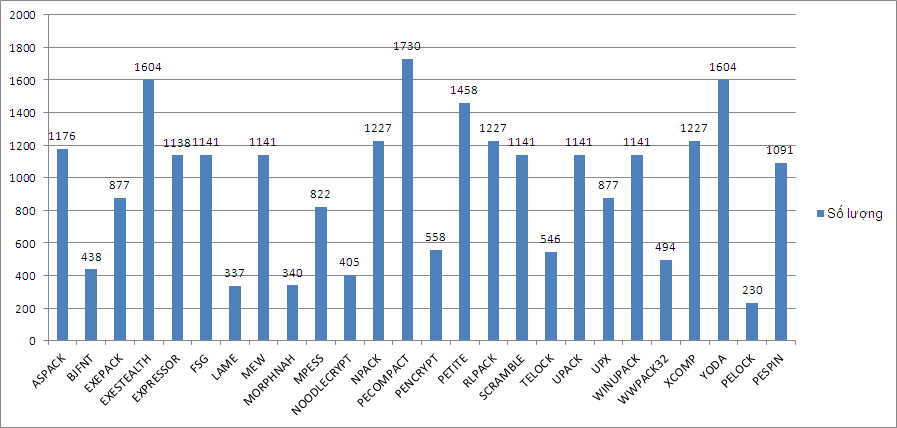
\includegraphics[width=0.8\textwidth]{packer_statistic}
\caption{Thống kê quá trình nhận dạng packer trên tập LORIA}
\label{fig:PackerStat}
\end{figure}

\hspace{0.5cm}Với kết quả thí nghiệm trên 2000 virus từ tập virus LORIA, hình \ref {fig:TechStat} thống kê số lượng từng kỹ thuật được packer sử dụng.

\begin{figure}
\centering
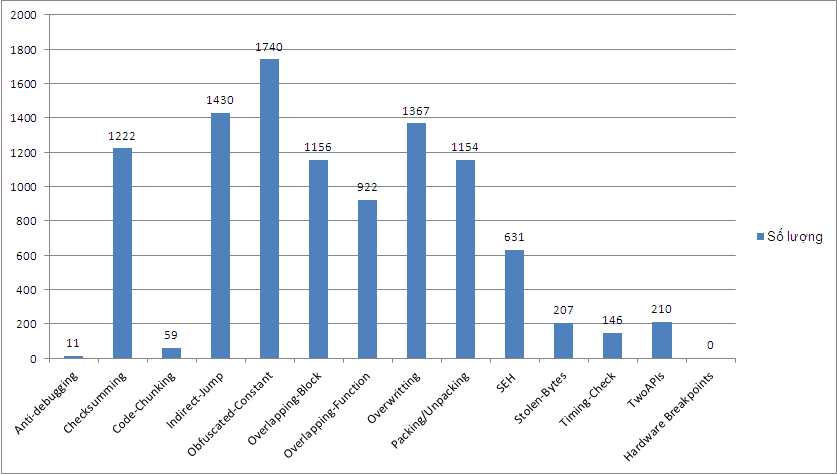
\includegraphics[width=0.8\textwidth]{technique_statistic}
\caption{Thống kê số lượng từng kỹ thuật của packer.}
\label{fig:TechStat}
\end{figure}

\section{Kết luận}

\hspace{0.5cm}Theo thống kê, số lượng những tập tin có kết quả nhận dạng packer thông qua chữ ký và thông qua ngữ nghĩa giống nhau là 335 trên tổng số 1942 malware được thí nghiệm. Điều này chứng tỏ quá trình nhận dạng thông qua ngữ nghĩa được thực hiện trong đề tài luận văn này còn những hạn chế nhất định và sẽ được cải tiến trong tương lai.\\

\hspace{0.5cm}Từ hình \ref {fig:TechStat} có thể thấy những kỹ thuật được sử dụng nhiều nhất trong packer là: Obfuscated Constants, Indirect Jump, Packing/Unpacking, Overwriting và Checksumming vốn là những kỹ thuật cốt lõi của packer.

